\documentclass[handout]{beamer}

\input{../Haust2015glærur}

\title{Tölvunarfræði 1a}
\subtitle{Vika 2, fyrri fyrirlestur}

\begin{document}

\begin{frame}
\titlepage
\end{frame}

\section{Inngangur}

\begin{frame}{Í síðasta þætti\ldots}
\begin{itemize}
 \item Slembitölur
 \item Kóðun bókstafa
 \item Röksegðir
\end{itemize}
\end{frame}

\subsection{Fyrri fyrirlestraæfingar}

\begin{frame}{Forritunarmálin sem þið kunnið}
\begin{center}
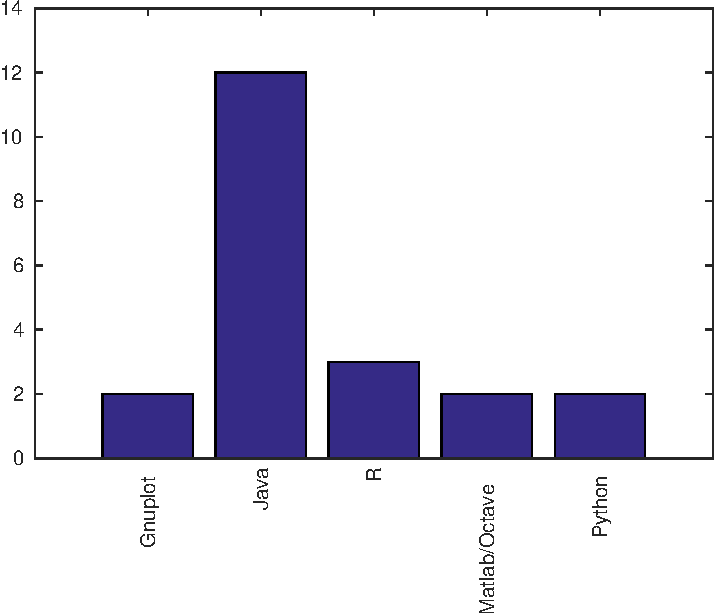
\includegraphics[width=0.7\textwidth]{Pics/forritunarmaladreifing}
\end{center}
\end{frame}

\begin{frame}{Forritunarmálin sem þið kunnið}
Annað sem komst á blað\pause
\begin{itemize}
 \item HTML/CSS
 \begin{itemize}
  \item Tæknilega ekki forritunarmál \pause
 \end{itemize}
 \item \LaTeX
 \begin{itemize}
  \item Tæknilega forritunarmál, venjulega ekki notað sem slíkt \pause
 \end{itemize}
 \item Man það ekki \pause
 \item C, Perl, Lisp, Go, PHP, Javascript, Haskell
\end{itemize}
\end{frame}

\begin{frame}{Gömul fyrirlestraræfing}
\begin{itemize}
 \item Spurningin: Hvers vegna gefur \texttt{round(rand()*10)} ekki jafndreifðar slembitölur? \pause
 \item Hugmynd að lausn:
 \begin{itemize}
  \item Við vitum (af fyrri glærum) að \texttt{rand()*10} gefur jafndreifðar slembi-kommutölur á bilinu $]0;10[$.
  \item Þegar \texttt{round(}\ldots\texttt{)} er tekið af því fást vissulega heiltölur á bilinu $[0;10]$\ldots
  \item En líklegra er að sumar komi upp en aðrar.
  \begin{itemize}
   \item $0$ kemur upp þegar \texttt{rand()*10} skilar gildi á bilinu $]0;0.5]$, $1$ á bilinu $[0.5;1.5[$, $2$ á bilinu $[1.5;2.5[$, o.s.frv.
   \item Bilin eru mislöng, svo tölurnar eru ekki jafndreifðar!
   \item Sama vandamál í kringum töluna 10
  \end{itemize}
 \end{itemize}
\end{itemize}
\end{frame}

\begin{frame}{Önnur gömul fyrirlestraræfingadæmi}
\begin{itemize}
 \item Hvaða sanngildi hefur yrðingin \texttt{3 > 2 > 1}?\pause
 \begin{itemize}
  \item Fyrst er \texttt{3 > 2} túlkað sem rökgildið $1$. Síðan er rökgildið $1$ borið saman við töluna $1$ líkt og það væri tala. $1$ er ekki stærri en $1$, svo heildarútkoman er $0$.
 \end{itemize} \pause
 \item Skrifið yrðingu sem er sönn þegar gildi breytunnar \texttt{a} er hvorki 0 né 10. \pause
 \begin{itemize}
  \item Skrifum fyrst tvær aðskildar yrðingar sem eru sannar þegar $a$ er ekki $0$ annars vegar og þegar $a$ er ekki $10$ hins vegar: \texttt{a \~{}= 0} er önnur og \texttt{a \~{}= 10} er hin.
  \item Tengjum þær svo saman með \texttt{\&\&}, svo heildarsegðin sé ósönn þegar önnur hvor segðanna er ósönn. \texttt{a \~{}= 0 \&\& a \~{}= 10}
 \end{itemize}
\end{itemize}
\end{frame}

\section{Hugtökin - vigrar og fylki}

\begin{frame}{Grundvallarhugtökin}
\begin{columns}
\column{0.5\textwidth}
\begin{itemize}
 \item Vigur (e. \emph{vector}) er röð minnishólfa geymd undir einu nafni (breytuheiti)
 \begin{itemize}
  \item Getum litið á það sem línuvigur (e. \emph{row vector}) eða dálkvigur (e. \emph{column vector})
 \end{itemize}
 \item Fylki (e. \emph{matrix}) er tvívíð tafla minnishólfa með sama nafni
\end{itemize}
\column{0.5\textwidth}
\begin{center}
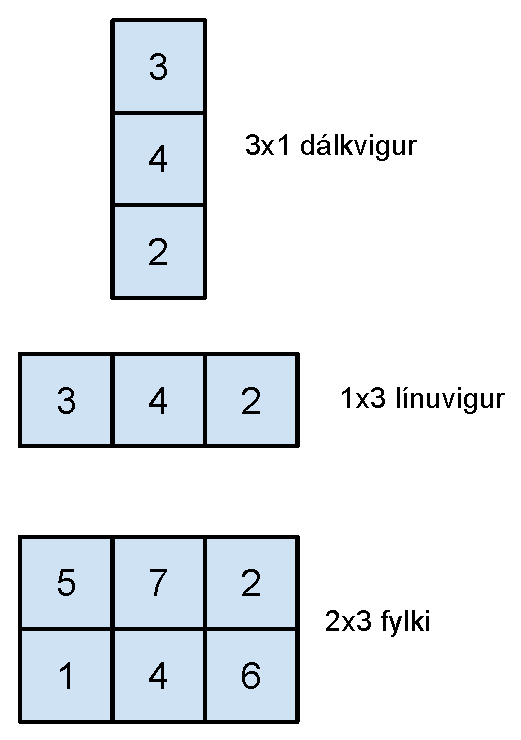
\includegraphics[height=0.8\textheight]{Pics/vigrar-og-fylki}
\end{center}
\end{columns}
\end{frame}

\subsection{Grundvallar-vigravinnsla}

\begin{frame}[fragile]{Að búa til vigra - bein upptalning}
\begin{columns}
\column{0.5\textwidth}
Búa má til vigra með því að telja upp gildin innan hornklofa
\begin{minted}[frame=lines]{matlab}
>> v = [8 32 17]
v =
     8    32    17
\end{minted} 
\column{0.5\textwidth}\pause
Jafngilt er að nota bil og kommur á milli staka í upptalningunni
\begin{minted}[frame=lines]{matlab}
>> v = [8, 32, 17]
v =
    8   32   17
\end{minted}
\end{columns}
\end{frame}

\begin{frame}[fragile]{Að búa til vigra - ``ítrun''}
\begin{columns}
\column{0.5\textwidth}
Nota má tvípunkt til þess að skilgreina bil gilda
\begin{minted}[frame=lines]{matlab}
>> v = 1:5
v =
   1   2   3   4   5
\end{minted}
\column{0.5\textwidth} \pause
Hægt er að tilgreina hversu langt á að vera á milli gildanna
\begin{minted}[frame=lines]{matlab}
>> 1:2:5
ans =
   1   3   5
\end{minted}
\end{columns}
\end{frame}

\begin{frame}[fragile]{Að vísa í stök vigra}
\begin{itemize}
 \item Stök vigra eru númeruð frá $1$
 \begin{itemize}
  \item Mörg önnur forritunarmál byrja á $0$
 \end{itemize}
 \item Hægt er að vísa í stök vigra með númerum þeirra
\begin{minted}[frame=lines]{matlab}
>> v = 6:10
v =
    6    7    8    9   10
>> v(2)
ans =  7
\end{minted}
\end{itemize}
\end{frame}

\begin{frame}[fragile]{Að vísa í mörg stök}
\begin{itemize}
 \item Nota má vigur til að vísa í vigur! (Fáum hlutvigur)
 \item Stökin sem svara til gilda vigursins eru þá sótt
\begin{minted}[frame=lines]{matlab}
>> v = 6:10
v =
    6    7    8    9   10
>> v(2:3) % 2:3 í sviganum býr til vigurinn [2, 3]
ans =
   7   8
\end{minted}
\end{itemize}
\end{frame}

\subsection{Dálkvigrar}

\begin{frame}[fragile]{Dálkvigrar}
\begin{itemize}
 \item Sjálfgefið er að búnir séu til línuvigrar
 \item Aðskilja má línur með \texttt{;} (semíkommu) til að búa til dálkvigra
\begin{minted}[frame=lines]{matlab}
>> cv = [1;2] % column vector
cv =
   1
   2
\end{minted}
\end{itemize}
\end{frame}

\begin{frame}[fragile]{Bylting}
\begin{columns}
\column{0.5\textwidth}
\begin{itemize}
 \item Breyta má línuvigri í dálkvigur og öfugt með \texttt{'} (komma uppi)
 \item Þetta er kallað að bylta (e. \emph{transpose}) vigrinum
 \begin{itemize}
  \item Bylting er venjulega táknuð með $A^T$ í línulegri algebru
 \end{itemize}
 \item Bylting virkar líka á fylki
\end{itemize}
\column{0.5\textwidth}
\begin{minted}[frame=lines]{matlab}
>> v = 1:2
v =
   1   2
>> v'
ans =
   1
   2
\end{minted}
\end{columns}
\end{frame}

\section{Fylki}

\begin{frame}[fragile]{Fylki}
\begin{itemize}
 \item Fylki eru búin til á svipaðan hátt og vigrar
 \item Fylki verða að hafa sama fjölda staka í öllum línum og öllum dálkum
\begin{minted}[frame=lines]{matlab}
>> b = [5, 7, 2; 1, 4, 6]
b =
   5   7   2
   1   4   6
>> bBroken = [5, 7, 2; 1, 4] % Gefur villu!
\end{minted}
\end{itemize}
\end{frame}

\begin{frame}{Gagnleg fylkjaföll}
\begin{center}
\begin{tabular}{ll}
\toprule
Fall&Niðurstaða\\
\midrule
\texttt{rand(n,m)}&$n\times m$ fylki með slembikommutölum \\
\texttt{randi([a,b], n)}&$n\times n$ fylki með slembiheiltölum á $[a;b]$\\
\texttt{zeros(n,m)}&$n \times m $ fylki með núllum\\
\texttt{ones(n,m)}&$n \times m $ fylki með ásum\\
\texttt{eye(n)}&$n \times n$ einingarfylki\\
\bottomrule
\end{tabular}
\end{center}
\end{frame}

\begin{frame}[fragile]{Vísun í stök fylkis}
\begin{columns}
\column{0.5\textwidth}
\begin{itemize}
 \item Vísa má í stök fylkis með því að gefa upp línunúmer og dálknúmer.
 \item Getum líka vísað í hlutfylki, svipað og með hlutvigur.
\end{itemize}
\column{0.5\textwidth}
\begin{minted}[frame=lines]{matlab}
>> b = [5, 7, 2; 1, 4, 6];
>> b(2,3)
ans =  6
>> b(2,2:3)
ans =
   4   6
>> b(1,:)
ans =
   5   7   2
\end{minted}
\end{columns}
\end{frame}

\begin{frame}[fragile]{Innsetning og eyðing lína/dálka}
\begin{columns}
\column{0.5\textwidth}
4. dálkinum bætt við
\begin{minted}[frame=lines]{matlab}
>> b = [5, 7, 2; 1, 4, 6];
>> b(:,4) = 1:2
b =
   5   7   2   1
   1   4   6   2
\end{minted}
\column{0.5\textwidth}
2. dálki eytt
\begin{minted}[frame=lines]{matlab}
>> b = b(:,[1, 3, 4])
b =
   5   2   1
   1   6   2
\end{minted}
\vspace{\baselineskip}
\end{columns}
\end{frame}

\begin{frame}[fragile]{Að lokum - lykilorðið end}
\begin{columns}
\column{0.5\textwidth}
Hægt er að vísa í síðasta stak vigurs með \texttt{end}
\begin{minted}[frame=lines]{matlab}
>> v = 1:8;
>> v(end)
ans =  8
\end{minted}
\column{0.5\textwidth}
Sömuleiðis hægt að vísa í síðustu línu eða dálk fylkis
\begin{minted}[frame=lines]{matlab}
>> b = [5, 7, 2; 1, 4, 6];
>> b(2,end)
ans =  6
\end{minted}
\end{columns}
\end{frame}

\begin{frame}{Fyrirlestraræfing}
\begin{enumerate}
 \item Hvaða vigur er skilgreindur með \texttt{7:-2:3}? (Hint: Skoðið \texttt{3:2:7})
 \item Búið til slembið $4 \times 4$ fylki með heiltölum á bilinu 5 til 20 og setjið í breytuna $a$
 \item Takið eitthvað $2 \times 2$ hlutfylki úr $a$ og setjið það í breytuna $b$
\end{enumerate}
\end{frame}

\subsection{Víddir fylkja}

\begin{frame}[fragile]{Víddir og stærðir}
\begin{columns}
\column{0.5\textwidth}
\begin{itemize}
 \item Fallið \texttt{size} gefur fjölda lína og dálka (víddir fylkisins)
 \item Fallið \texttt{length} gefur stærri töluna sem \texttt{size} skilar
 \begin{itemize}
  \item Sem sagt, lengd vigurs
 \end{itemize}
 \item \texttt{numel(x)} gefur fjölda staka
\end{itemize}
\column{0.5\textwidth}
\begin{minted}[frame=lines]{matlab}
>> b = [5, 7, 2; 1, 4, 6];
>> size(b)
ans = 
    2    3
>> length(5:5:50)
ans = 
    10
\end{minted}
\end{columns}
\end{frame}

\begin{frame}[fragile]{Endurröðun lína og dálka}
\vspace{\baselineskip}
Föllin \texttt{fliplr} (flip left-right) og \texttt{flipud} (flip up-down) snúa við röð dálka og lína
\begin{columns}
\column{0.5\textwidth}
\begin{minted}[frame=lines]{matlab}
>> a = [1, 2; 3, 4]
a =
   1   2
   3   4
>> fliplr(a)
ans =
   2   1
   4   3
\end{minted}
\column{0.5\textwidth}
\begin{minted}[frame=lines]{matlab}
>> a = [1, 2; 3, 4]
a =
   1   2
   3   4
>> flipud(a)
ans =
   3   4
   1   2
\end{minted}
\end{columns}
\end{frame}

\begin{frame}[fragile]{Snúningur}
\vspace{\baselineskip}
Fallið \texttt{rot90} snýr stökum fylkis rangsælis um $90^\circ$. Hægt er að fá snúning um $k\cdot90^\circ$ með viðfangi $k$ í fallið.
\begin{columns}
\column{0.5\textwidth}
\begin{minted}[frame=lines]{matlab}
>> a = [1, 2; 3, 4];
>> rot90(a)
ans =
   2   4
   1   3
\end{minted}
\column{0.5\textwidth}
\begin{minted}[frame=lines]{matlab}
>> a = [1, 2; 3, 4];
>> rot90(a,2)
ans =
   4   3
   2   1
\end{minted}
\end{columns}
\vspace{\baselineskip}
Helst er þetta notað þegar fylkið táknar mynd.
\end{frame}

\section{Notkun falla á fylki}

\begin{frame}[fragile]{Notkun falla með vigrum og fylkjum}
Mörg föll í Matlab eru fær um að taka við vigrum og fylkjum af gildum. Fallinu er þá oftast beitt á hvert stak fyrir sig.
\begin{minted}[frame=lines]{matlab}
>> 0:4:16
ans =
    0    4    8   12   16
>> sqrt(ans)
ans =
   0.00000   2.00000   2.82843   3.46410   4.00000
\end{minted}
\end{frame}

\section{Tómir vigrar og eyðing}

\begin{frame}[fragile]{Tómir vigrar}
Búa má til tóma vigra
\begin{minted}[frame=lines]{matlab}
>> ev = []
ev = []
\end{minted}
Síðan má bæta við stökum eftirá
\begin{minted}[frame=lines]{matlab}
>> ev = [ev, 5]
ev =  5
>> ev = [ev, 8]
ev =
   5   8
\end{minted}
Þetta er þó ekki sérstaklega skilvirk aðferð (meira síðar)
\end{frame}

\begin{frame}[fragile]{Eyðing staka}
\begin{columns}
\column{0.5\textwidth}
Nota má tóma vigra til að eyða stökum
\begin{minted}[frame=lines]{matlab}
>> v = 1:5;
>> v(3) = []
v =
   1   2   4   5

\end{minted}
\column{0.5\textwidth}
Eyða má mörgum stökum í einu
\begin{minted}[frame=lines]{matlab}
>> v = 1:5;
>> v(1:2) = []
v =
   3   4   5
\end{minted}
\end{columns}
\vspace{\baselineskip}
Ath. að vegna þess að jafn mörg stök verða að vera í hverri línu og hverjum dálki er ekki hægt að eyða einstökum stökum úr fylkjum. Eyða þarf heilli línu eða heilum dálki í einu.
\end{frame}

\section{Margvíð fylki}

\begin{frame}[fragile]{Margvíð föll}
\begin{columns}
\column{0.5\textwidth}
Hægt er að búa til fylki af meira en tveimur víddum (þrívíð, fjórvíð, $n$-víð)
\begin{minted}[frame=lines]{matlab}
>> a = ones(2,3,2)
a =
ans(:,:,1) =
   1   1   1
   1   1   1
ans(:,:,2) =
   1   1   1
   1   1   1
\end{minted}
\column{0.5\textwidth}
\begin{itemize}
 \item Hér er fylkið $a$ þrívítt, með víddir $2$, $3$ og $2$
 \item Fylkið er hér sýnt ``lag fyrir lag''
 \item \texttt{ones}, \texttt{zeros} og \texttt{rand} virka öll til að gera margvíð fylki
\end{itemize}
\end{columns}
\end{frame}

\section{Föll fyrir fylki og vigra}

\begin{frame}[fragile]{Föll fyrir vigra}
\begin{columns}
\column{0.5\textwidth}
\begin{itemize}
 \item Mörg Matlab-föll virka ``stakvíst'' á vigra og fylki
 \begin{itemize}
  \item Eitt stak meðhöndlað í einu
 \end{itemize}
 \item Sum föll eru sérstaklega hönnuð fyrir vigra og/eða fylki sem heild, t.d. \texttt{min} og \texttt{sum}
 \item Fleiri föll sem eru hentug fyrir vigra: \texttt{max}, \texttt{cumsum}, \texttt{prod}
\end{itemize}
\column{0.5\textwidth}
\begin{minted}[frame=lines]{matlab}
>> v = [3 5 8 8 2 4];
>> min(v)
ans =  2
>> sum(v)
ans =  30
\end{minted}
\end{columns}
\end{frame}

\begin{frame}[fragile]{Vigurföll notuð á fylki}

Þegar fall sem ætlað er til nota á vigur er notað á fylki virkar það á hvern \emph{dálk} fylkisins fyrir sig.

\begin{minted}[frame=lines]{matlab}
>> a = [3 5 8; 8 2 4];
>> max(a)
ans =
   8   5   8
>> sum(a)
ans =
   11    7   12
\end{minted}
\end{frame}

\begin{frame}{Fyrirlestraræfing}
\begin{enumerate}
\setcounter{enumi}{3}
 \item Gefinn er vigurinn \texttt{v = 1:10}. Sýnið eina Matlab-skipun sem eyðir öllum oddatölunum úr vigrinum (Hægt er að gera þetta án þess að telja upp stökin eitt í einu!)
 \item Búið til slembið $3 \times 3$ fylki af heiltölum á bilinu $[1:10]$ og geymið það í breytunni $a$. Finnið summu allra staka í fylkinu
 \item Finnið minnstu summu \emph{lína} í fylkinu $a$, sem búið var til í fyrri lið
\end{enumerate}
\end{frame}




\end{document}
